\documentclass[a4paper, 11pt]{article}
\usepackage{graphicx}
\usepackage{multicol}
\usepackage{tabularx}
\usepackage{enumitem}
\usepackage[a4paper, margin=1.8cm]{geometry}
\usepackage{listings}
\usepackage{amssymb}
\usepackage{gvv}
\usepackage{gvv-book}
\usepackage{amsmath}
\usepackage{setspace}
\usepackage{caption}

\graphicspath{ {./figs/} }

\begin{document}
\begin{center}
    \huge{CS: COMPUTER SCIENCE AND INFORMATION TECHNOLOGY}\\
    \large{EE25BTECH11041 - Naman Kumar}
\end{center}

\begin{enumerate}
    \item The statement $(\neg p)\Rightarrow(\neg q)$ is logically equivalent to which of the statements below?
    \begin{enumerate}[label=\Roman*]
        \item $p\Rightarrow q$ 
        \item $q\Rightarrow p$
        \item $(\neg q)\vee p$
        \item $(\neg p)\vee q$
    \end{enumerate}
    
    \begin{enumerate}
    \begin{multicols}{4}
        \item I only
        \item I and IV only
        \item II only
        \item II and III only
    \end{multicols}
    \end{enumerate}
    
    \hfill (GATE CS 2017)
    
    \item Consider the first-order logic sentence $F\colon \forall x(\exists y~R(x,y))$. Assuming non-empty logical domains, which of the sentences below are implied by $F$?
    \begin{enumerate}[label=\Roman*]
        \item $\exists y(\exists xR(x,y))$
        \item $\exists v(\forall xR(x,y))$
        \item $\forall y(\exists xR(x,y))$
        \item $\neg\exists x(\forall y\neg R(x,y))$
    \end{enumerate}
    
    \begin{enumerate}
    \begin{multicols}{4}
        \item IV only
        \item I and IV only
        \item II only
        \item II and III only
        \end{multicols}
    \end{enumerate}
    
    \hfill (GATE CS 2017)
    
    \item Let $c_{1},...,c_{n}$ be scalars, not all zero, such that $\sum_{i=1}^{n}c_{i}a_{i}=0$ where $a_{i}$ are column vectors in $R^{n}$. Consider the set of linear equations \\$Ax=b$ \\where $A=[a_{1},...,a_{n}]$ and $b=\sum_{i=1}^{n}a_{i}$. The set of equations has
    
    \begin{enumerate}
        \item a unique solution at $x=J_{n}$ where $J_{n}$ denotes a 11-dimensional vector of all 1
        \item no solution
        \item infinitely many solutions
        \item finitely many solutions
    \end{enumerate}
    
    \hfill (GATE CS 2017)
    
    \item Consider the following functions from positive integers to real numbers:\\ $10, \sqrt{n}, n, \log_{2}n, \frac{100}{n}$.\\ The CORRECT arrangement of the above functions in increasing order of asymptotic complexity is:
    
    \begin{enumerate}
        \begin{multicols}{2}
            \item $\log_{2}n, \frac{100}{n}, 10, \sqrt{n}, n$
            \item $\frac{100}{n}, 10, \log_{2}n, \sqrt{n}, n$
            \item $10, \frac{100}{n}, \sqrt{n}, \log_{2}n, n$
            \item $\frac{100}{n}, \log_{2}n, 10, \sqrt{n}, n$
        \end{multicols}
    \end{enumerate}
    
    \hfill (GATE CS 2017)
    
    \item Consider the following table:
    
    \begin{tabular}{|c|c|}
        \hline
        \textbf{Algorithms} & \textbf{Design Paradigms} \\
        \hline
        (P) Kruskal & (i) Divide and Conquer \\
        (Q) Quicksort & (ii) Greedy \\
        (R) Floyd-Warshall & (iii) Dynamic Programming \\
        \hline
    \end{tabular}
    
    Match the algorithms to the design paradigms they are based on.
    
    \begin{enumerate}
        \item (P)$\leftrightarrow$(ii), (Q)$\leftrightarrow$(iii), (R)$\leftrightarrow$(i)
        \item (P)$\leftrightarrow$(iii), (Q)$\leftrightarrow$(i), (R)$\leftrightarrow$(ii)
        \item (P)$\leftrightarrow$(ii), (Q)$\leftrightarrow$(i), (R)$\leftrightarrow$(iii)
        \item (P)$\leftrightarrow$(i), (Q)$\leftrightarrow$(ii), (R)$\leftrightarrow$(iii)
    \end{enumerate}
    
    \hfill (GATE CS 2017)
    
    \item Let T be a binary search tree with 15 nodes. The minimum and maximum possible heights of T are: \textit{Note: The height of a tree with a single node is 0.}
    
    \begin{enumerate}
    \begin{multicols}{2}
        \item 4 and 15 respectively
        \item 3 and 14 respectively
        \item 4 and 14 respectively
        \item 3 and 15 respectively
        \end{multicols}
    \end{enumerate}
    
    \hfill (GATE CS 2017)
    
    \item The n-bit fixed-point representation of an unsigned real number X uses f bits for the fraction part. Let $i=n-f$. The range of decimal values for X in this representation is
    
    \begin{enumerate}
    \begin{multicols}{4}
        \item $2^{-f}$ to $2^{i}$
        \item $2^{-f}$ to $(2^{i}-2^{-f})$
        \item 0 to $2^{i}$
        \item 0 to $(2^{i}-2^{-i})$
        \end{multicols}
    \end{enumerate}
    
    \hfill (GATE CS 2017)
    
    \item Consider the C code fragment given below.
    
    \begin{lstlisting}[language=C]
    typedef struct node {
        int data;
        struct node* next;
    } node;
    
    void join (node* m, node* n) {
        node* p = n;
        while (p->next != NULL) {
            p = p->next;
        }
        p->next = m;
    }
    \end{lstlisting}
    
    Assuming that m and n point to valid NULL-terminated linked lists, invocation of join will
    
    \begin{enumerate}
        \item append list m to the end of list n for all inputs.
        \item either cause a null pointer dereference or append list m to the end of list n.
        \item cause a null pointer dereference for all inputs.
        \item append list n to the end of list m for all inputs.
    \end{enumerate}
    
    \hfill (GATE CS 2017)
    
    \item When two 8-bit numbers $A_{7}\cdot\cdot\cdot A_{0}$ and $B_{7}\cdot\cdot\cdot B_{0}$ in 2's complement representation (with $A_{0}$ and $B_{0}$ as the least significant bits) are added using a ripple-carry adder, the sum bits obtained are $S_{7}\cdot\cdot\cdot S_{0}$ and the carry bits are $C_{7}\cdot\cdot\cdot C_{0}$. An overflow is said to have occurred if
    
    \begin{enumerate}
        \item the carry bit $C_{7}$ is 1
        \item all the carry bits $(C_{7},\cdot\cdot\cdot,C_{0})$ are 1
        \item $(A_{7}\cdot B_{7}\cdot\overline{S_{7}}+\overline{A_{7}}\cdot\overline{B_{7}}\cdot S_{7})$ is 1
        \item $(A_{0}\cdot B_{0}\cdot\overline{S_{0}}+\overline{A_{0}}\cdot\overline{B_{0}}\cdot S_{0})$ is 1
    \end{enumerate}
    
    \hfill (GATE CS 2017)
    
    \item Consider the following context-free grammar over the alphabet $\Sigma=\{a,b,c\}$ with S as the start symbol:\\ $S\rightarrow abScT|abcT$\\$T\rightarrow bT|b$\\
    Which one of the following represents the language generated by the above grammar?
    \begin{enumerate}
        \item $\{(ab)^{n}(cb)^{n}|n\ge1\}$
        \item $\{(ab)^{n}cb^{m_{1}}cb^{m_{2}}...cb^{m_{n}}|n,m_{1},m_{2},...,m_{n}\ge1\}$
        \item $\{(ab)^{n}(cb^{m})^{n}|m,n\ge1\}$
        \item $\{(ab)^{n}(cb^{n})^{m}|m,n\ge1\}$
    \end{enumerate}
    
    \hfill (GATE CS 2017)
    
    \item Consider the C struct defined below:
    
    \begin{lstlisting}[language=C]
    struct data {
        int marks [100];
        char grade;
        int cnumber;
    };
    struct data student;
    \end{lstlisting}
    
    The base address of student is available in register R1. The field student.grade can be accessed efficiently using
    
    \begin{enumerate}
        \item Post-increment addressing mode. (R1)+
        \item Pre-decrement addressing mode. - (R1)
        \item Register direct addressing mode. R1
        \item Index addressing mode. X(R1) where X is an offset represented in 2's complement 16-bit representation.
    \end{enumerate}
    
    \hfill (GATE CS 2017)
    
    \item Consider the following intermediate program in three address code
    $p=a-b$\\
    $q=p*c$\\
    $p=u*v$\\
    $q=p+q$\\
    Which one of the following corresponds to a static single assignment form of the above code?
    
    \begin{enumerate}
        \begin{multicols}{2}
            \item $p_{1}=a-b$\\
            $q_{1}=p_{1}*c$\\
            $p_{1}=u*v$\\
            $q_{1}=p_{1}+q_{1}$
            \item $p_{3}=a-b$\\
            $q_{4}=p_{3}*c$\\
            $p_{4}=u*v$\\
            $q_{5}=p_{4}+q_{4}$
            \item $p_{1}=a-b$\\
            $q_{1}=p_{2}*c$\\
            $p_{3}=u*v$\\
            $q_{2}=p_{4}+q_{3}$
            \item $p_{1}=a-b$\\
            $q_{1}=p*c$\\
            $p_{2}=u*v$\\
            $q_{2}=p+q$
        \end{multicols}
    \end{enumerate}
    
    \hfill (GATE CS 2017)
    
    \item Consider the following C code:
    
    \begin{lstlisting}[language=C]
    #include <stdio.h>
    #include <stdlib.h>
    
    int *assignval (int *x, int val) {
        *x = val;
        return x;
    }
    
    void main () {
        int *x = malloc(sizeof(int));
        if (NULL == x) return;
    
        x = assignval(x,0);
        
        if(x) {
            x = (int *)malloc(sizeof(int));
            if (NULL == x) return;
            x = assignval(x,10);
            printf("%d\n", *x);
            free(x);
        }
    }
    \end{lstlisting}
    
    The code suffers from which one of the following problems:
    
    \begin{enumerate}
        \item compiler error as the return of malloc is not typecast appropriately
        \item compiler error because the comparison should be made as $x==$ NULL and not as shown
        \item compiles successfully but execution may result in dangling pointer
        \item compiles successfully but execution may result in memory leak
    \end{enumerate}
    
    \hfill (GATE CS 2017)
    
    \item Consider a TCP client and a TCP server running on two different machines. After completing data transfer, the TCP client calls close to terminate the connection and a FIN segment is sent to the TCP server. Server-side TCP responds by sending an ACK, which is received by the client-side TCP. As per the TCP connection state diagram (RFC 793), in which state does the client-side TCP connection wait for the FIN from the server-side TCP?
    
    \begin{enumerate}
    \begin{multicols}{4}
        \item LAST-ACK
        \item TIME-WAIT
        \item FIN-WAIT-1
        \item FIN-WAIT-2
        \end{multicols}
    \end{enumerate}
    
    \hfill (GATE CS 2017)
    
    \item A sender S sends a message m to receiver R, which is digitally signed by S with its private key. In this scenario, one or more of the following security violations can take place.
    \begin{enumerate}[label=\Roman*]
        \item S can launch a birthday attack to replace m with a fraudulent message.
        \item A third party attacker can launch a birthday attack to replace m with a fraudulent message.
        \item R can launch a birthday attack to replace m with a fraudulent message.
    \end{enumerate}
    Which of the following are possible security violations?
    
    \begin{enumerate}
        \item (I) and (II) only
        \item (I) only
        \item (II) only
        \item (II) and (III) only
    \end{enumerate}
    
    \hfill (GATE CS 2017)
    
    \item The following functional dependencies hold true for the relational schema R{V, W, X, Y, Z}:
    \begin{center}
        $V\rightarrow W$\\
        $VW\rightarrow X$\\
        $Y\rightarrow VX$\\
        $Y\rightarrow Z$
    \end{center}
    Which of the following is irreducible equivalent for this set of functional dependencies?
    
    \begin{enumerate}
        \begin{multicols}{4}
            \item $V\rightarrow W\\V\rightarrow X\\Y\rightarrow V \\Y\rightarrow Z$
            \item $V\rightarrow W\\ W\rightarrow X\\ Y\rightarrow V\\ Y\rightarrow Z$
            \item $V\rightarrow W\\ V\rightarrow X\\ Y\rightarrow V\\ Y\rightarrow X,\\ Y\rightarrow Z$
            \item $V\rightarrow W\\ W\rightarrow X\\ Y\rightarrow V\\ Y\rightarrow X\\Y\rightarrow Z$
        \end{multicols}
    \end{enumerate}
    
    \hfill (GATE CS 2017)
    
    \item Consider the following grammar:\\
    $P \rightarrowx QRS$\\
    $Q\rightarrow yz | z$\\
    $R\rightarrow w | \varepsilon$\\
    $S\rightarrow y$\\
    What is FOLLOW(Q)?
    
    \begin{enumerate}
        \begin{multicols}{4}
            \item $\{R\}$
            \item $\{w\}$
            \item $\{w, y\}$
            \item $\{w, \$\}$
        \end{multicols}
    \end{enumerate}
    
    \hfill (GATE CS 2017)
    
    \item Threads of a process share
    
    \begin{enumerate}
        \item global variables but not heap.
        \item heap but not global variables.
        \item neither global variables nor heap.
        \item both heap and global variables.
    \end{enumerate}
    
    \hfill (GATE CS 2017)
    
    \item Let X be a Gaussian random variable with mean 0 and variance $\sigma^{2}$. Let $Y=\max(X,0)$ where $\max(a,b)$ is the maximum of a and b. The median of Y is \underline{\hspace{2cm}}.
    
    \hfill (GATE CS 2017)
    
    \item Let T be a tree with 10 vertices. The sum of the degrees of all the vertices in T is \underline{\hspace{2cm}}.
    
    \hfill (GATE CS 2017)
    
    \item Consider the Karnaugh map given below, where X represents “don’t care” and blank represents 0.
    
    \begin{figure}[H]
        \centering
        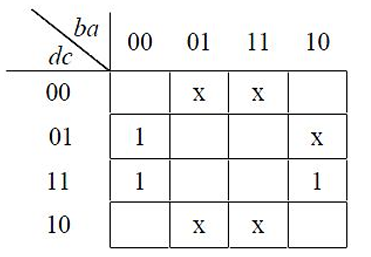
\includegraphics[width=5cm, ]{figs/q21.png}
        \label{fig:placeholder}
    \end{figure}
    
    Assume for all inputs (a,b,c,d). the respective complements $(\vec{a},\vec{b}, \vec{c}, \vec{d})$ are also available. The  above logic is implemented using 2-input NOR gates only. The minimum number of gates required  is \underline{\hspace{2cm}}.
    
    \hfill (GATE CS 2017)
    
    \item Consider the language L given by the regular expression $(a+b)^{*}b(a+b)^{*}$ over the alphabet $\{a,b\}$. The smallest number of states needed in a deterministic finite-state automaton (DFA) accepting L is \underline{\hspace{2cm}}.
    
    \hfill (GATE CS 2017)
    
    \item Consider a database that has the relation schema EMP (EmpId, EmpName, DeptName). An instance of the schema EMP and a SQL query on it are given below.\\
    \begin{minipage}[t]{0.48\textwidth}
        \begin{tabular}{|c|c|c|}
        \hline
        \multicolumn{3}{|c|}{EMP}\\
        \hline
        EmpId & EmpName & DeptName \\
        \hline
         1 & XYA & AA \\
         2 & XYB & AA \\
         3 & XYC & AA \\
         4 & XYD & AA \\
         5 & XYE & AB \\
         6 & XYF & AB \\
         7 & XYG & AC \\
         8 & XYH & AC \\
         9 & XYI & AC \\
         10 & XYJ & AC \\
         11 & XYK & AD \\
         12 & XYL & AD \\
         13 & XYM & AE \\
        \hline
    \end{tabular}
    \end{minipage}
    \begin{minipage}[t]{0.48\textwidth}
        \begin{lstlisting}
    SELECT AVG(EC.Num)
    FROM EC WHERE (DeptName, Num) IN
        (SELECT DeptName, COUNT(EmpId) AS 
                    EC(DeptName, Num)
        FROM EMP 
        GROUP BY DeptName)
    \end{lstlisting}
    \end{minipage}
    
    
    The output of executing the SQL query is \underline{\hspace{2cm}}.
    
    \hfill (GATE CS 2017)
    
    \item Consider the following CPU processes with arrival times (in milliseconds) and length of CPU bursts (in milliseconds) as given below:
    \begin{center}
    \begin{tabular}{|c|c|c|}
        \hline
        Process & Arrival time & Burst time \\
        \hline
        P1 & 0 & 7 \\
        P2 & 3 & 3 \\
        P3 & 5 & 5 \\
        P4 & 6 & 2 \\
        \hline
    \end{tabular}
    \end{center}
    
    If the pre-emptive shortest remaining time first scheduling algorithm is used to schedule the processes, then the average waiting time across all processes is \underline{\hspace{2cm}} milliseconds.
    
    \hfill (GATE CS 2017)
    
     \item Consider a two-level cache hierarchy with L1 and L2 caches. An application incurs 1.4 memory accesses per instruction on average. For this application, the miss rate of L1 cache is 0.1; the L2 cache experiences, on average, 7 misses per 1000 instructions. The miss rate of L2 expressed correct to two decimal places is \underline{\hspace{2cm}}
    
    \hfill{\brak{\text{GATE CS 2017}}}
    
    \item Let $G=\brak{V,E}$ be any connected undirected edge-weighted graph. The weights of the edges in E are positive and distinct. Consider the following statements:
    \begin{enumerate}[label=\Roman*]
        \item Minimum Spanning Tree of G is always unique.
        \item Shortest path between any two vertices of G is always unique.
    \end{enumerate}
    
    
    Which of the above statements is/are necessarily true?
    \begin{enumerate}
        \item I only
        \item II only
        \item both I and II
        \item neither I nor II
    \end{enumerate}

    \hfill{\brak{\text{GATE CS 2017}}}

    \item A multithreaded program P executes with x number of threads and uses y number of locks for ensuring mutual exclusion while operating on shared memory locations. All locks in the program are non-reentrant. \brak{\text{i.e., if a thread holds a lock l, then it cannot re-acquire lock l without releasing it}}. If a thread is unable to acquire a lock, it blocks until the lock becomes available. The minimum value of x and the minimum value of y together for which execution of P can result in a deadlock are:
    \begin{enumerate}
        \begin{multicols}{2}
            \item $x=1, y=2$
            \item $x=2, y=1$
            \item $x=2, y=2$
            \item $x=1, y=1$
        \end{multicols}
    \end{enumerate}

    \hfill{\brak{\text{GATE CS 2017}}}

    \item The value of {\Large$\lim_{x\to1}\frac{x^{7}-2x^{5}+1}{x^{3}-3x^{2}+2}$}
    \begin{enumerate}
    \begin{multicols}{4}
        \item is $0$
        \item is $-1$
        \item is $1$
        \item does not exist
    \end{multicols}
    \end{enumerate}
    
    \hfill{\brak{\text{GATE CS 2017}}}
    
    \item Let p, q, and r be propositions and the expression $\brak{p\to q}\to r$ be a contradiction. Then, the expression $\brak{r\to p}\to q$ is
    \begin{enumerate}
        \begin{multicols}{2}
            \item a tautology.
            \item a contradiction.
            \item always TRUE when p is FALSE.
            \item always TRUE when q is TRUE.
        \end{multicols}
    \end{enumerate}
    
    \hfill{\brak{\text{GATE CS 2017}}}

    \item Let u and v be two vectors in $R^{2}$ whose Euclidean norms satisfy $\abs{\abs{u}}=2\abs{\abs{v}}$. What is the value of $\alpha$ such that $w=u+\alpha v$ bisects the angle between u and v?
    \begin{enumerate}
        \begin{multicols}{2}
            \item $2$
            \item $1/2$
            \item $1$
            \item $-1/2$
        \end{multicols}
    \end{enumerate}
    
    \hfill{\brak{\text{GATE CS 2017}}}

    \item Let A be $n\times n$ real valued square symmetric matrix of rank 2 with $\sum_{i=1}^{n}\sum_{j=1}^{n}A_{ij}^{2}=50.$ Consider the following statements.
    \begin{enumerate}[label=\Roman*]
        \item One eigenvalue must be in $\brak[-5, 5]$
        \item The eigenvalue with the largest magnitude must be strictly greater than $5$
    \end{enumerate}
    
    Which of the above statements about eigenvalues of A is/are necessarily CORRECT?
    \begin{enumerate}
        \item Both I and II
        \item I only
        \item II only
        \item Neither I nor II
    \end{enumerate}
    
    \hfill{\brak{\text{GATE CS 2017}}}

    \item A computer network uses polynomials over $GF\brak{2}$ for error checking with 8 bits as information bits and uses $x^{3}+x+1$ as the generator polynomial to generate the check bits. In this network, the message 01011011 is transmitted as
    \begin{enumerate}
        \begin{multicols}{2}
            \item 01011011010
            \item 01011011011
            \item 01011011101
            \item 01011011100
        \end{multicols}
    \end{enumerate}
    
    \hfill{\brak{\text{GATE CS 2017}}}

    \item Consider a combination of T and D flip-flops connected as shown below. The output of the D flip-flop is connected to the input of the T flip-flop and the output of the T flip-flop is connected to the input of the D flip-flop.
    
    \begin{figure}[h]
        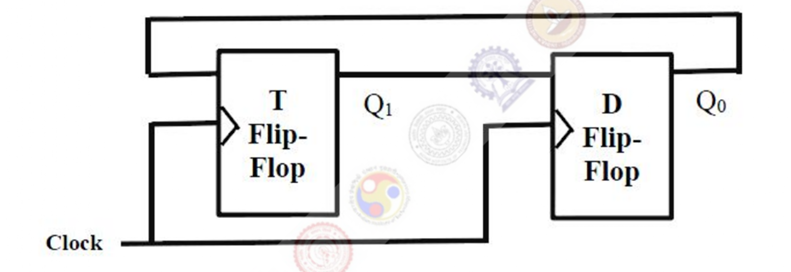
\includegraphics[width=\columnwidth]{figs/q33.png}
        \label{fig:placeholder}
    \end{figure}
    
    Initially, both $Q_{0}$ and $Q_{1}$ are set to $1$ \brak{\text{before the $1^{st}$ clock cycle}}. The outputs $Q_{1}Q_{0}$ after the $3^{rd}$ cycle are 11 and after the $4^{th}$ cycle are 00 respectively.
    \begin{enumerate}
        \item $Q_{1}Q_{0}$ after the $3^{rd}$ cycle are $11$ and after the $4^{th}$ cycle are $00$ respectively
        \item $Q_{1}Q_{0}$ after the $3^{rd}$ cycle are $11$ and after the $4^{th}$ cycle are $01$ respectively
        \item $Q_{1}Q_{0}$ after the $3^{rd}$ cycle are $00$ and after the $4^{th}$ cycle are $11$ respectively
        \item $Q_{1}Q_{0}$ after the $3^{rd}$ cycle are $01$ and after the $4^{th}$ cycle are $01$ respectively
    \end{enumerate}
    
    \hfill{\brak{\text{GATE CS 2017}}}

    \item If G is a grammar with productions
    \begin{center}
        $S\to SaS|aSb|bSa|SS|\epsilon$
    \end{center}
    where S is the start variable, then which one of the following strings is not generated by G?
    \begin{enumerate}
        \begin{multicols}{4}
            \item abab
            \item aaab
            \item abbaa
            \item babba
        \end{multicols}
    \end{enumerate}
    
    \hfill{\brak{\text{GATE CS 2017}}}

    \item Consider the following two functions.\\
    \begin{minipage}{5cm}
    \begin{lstlisting}
        void funl (int n) {
            if (n==0) return;
            printf("%d", n);
            fun2 (n - 2);
            printf("%d", n);
        }
    \end{lstlisting}
    
    \end{minipage}
    \begin{minipage}{5cm}
    \begin{lstlisting}
            void fun2 (int n) {
            if (n==0) return;
            printf("%d", n);
            funl (++n);
            printf("%d", n);
        }
    \end{lstlisting}
    
    \end{minipage}
        
    
    The output printed when fun1\brak{5} is called is
    \begin{enumerate}
        \begin{multicols}{2}
            \item 53423122233445
            \item 53423120112233
            \item 53423122132435
            \item 53423120213243
        \end{multicols}
    \end{enumerate}
    
    \hfill{\brak{\text{GATE CS 2017}}}

    \item Consider the C functions foo and bar given below:
    \begin{verbatim}
        int foo (int val) {
            int x=0;
            while (val > 0) {
                x = x + foo(val--);
            }
            return val;
        }

        int bar (int val) {
            int x=0;
            while (val > 0) {
                x = x + bar(val-1);
            }
            return val;
        }
    \end{verbatim}
    Invocations of foo\brak{3} and bar\brak{3} will result in :
    \begin{enumerate}
        \item Return of $6$ and $6$ respectively.
        \item Infinite loop and abnormal termination respectively.
        \item Abnormal termination and infinite loop respectively.
        \item Both terminating abnormally.
    \end{enumerate}
    
    \hfill{\brak{\text{GATE CS 2017}}}

    \item Consider the context-free grammars over the alphabet $\{a, b, c\}$ given below. S and T are non-terminals.\\
    $G_{1}:S\to aSb|T, T\to cT|\epsilon$
    $G_{2}:S\to bSa|T, T\to cT|\epsilon$\\
    The language $L\brak{G_{1}}\cap L\brak{G_{2}}$ is
    \begin{enumerate}
    \begin{multicols}{2}
        \item Finite.
        \item Not finite but regular.
        \item Context-Free but not regular.
        \item Recursive but not context-free.
    \end{multicols}
    \end{enumerate}
    
    \hfill{\brak{\text{GATE CS 2017}}}

    \item Consider the following languages over the alphabet $\Sigma=\{a,b,c\}$
    Let $L_{1}=\{a^{n}b^{n}c^{m}|m,n\ge0\}$ and $L_{2}=\{a^{m}b^{n}c^{n}|m,n\ge0\}$.
    
    Which of the following are context-free languages?
    \begin{enumerate}[label=\Roman*]
        \item $L_{1}\cup L_{2}$
        \item $L_{1}\cap L_{2}$
    \end{enumerate}    
    \begin{enumerate}
        \begin{multicols}{2}
            \item I only
            \item II only
            \item I and II
            \item Neither I nor II
        \end{multicols}
    \end{enumerate}
    
    \hfill{\brak{\text{GATE CS 2017}}}

    \item Let A and B be finite alphabets and let \# be a symbol outside both A and B. Let f be a total function from $A^{*}$ to $B^{*}$. We say f is computable if there exists a Turing machine M which given an input x in $A^{*}$, always halts with $f\brak{x}$ on its tape.
    Let $L_{f}$ denote the language $\{x\#f\brak{x}|x\in A^{*}\}$. Which of the following statements is true:
    \begin{enumerate}
        \item f is computable if and only if $L_{f}$ is recursive.
        \item f is computable if and only if $L_{f}$ is recursively enumerable.
        \item If f is computable then $L_{f}$ is recursive, but not conversely.
        \item If f is computable then $L_{f}$ is recursively enumerable but not conversely.
    \end{enumerate}
    
    \hfill{\brak{\text{GATE CS 2017}}}

    \item Recall that Belady's anomaly is that the page-fault rate may increase as the number of allocated frames increases. Now, consider the following statements:
    \begin{center}
    S1: Random page replacement algorithm \brak{\text{where a page chosen at random is replaced}} suffers from Belady's anomaly.
    
    S2: LRU page replacement algorithm suffers from Belady's anomaly.
    \end{center}
    
    Which of the following is CORRECT?
    \begin{enumerate}
        \begin{multicols}{2}
            \item S1 is true, S2 is true
            \item S1 is true, S2 is false
            \item S1 is false, S2 is true
            \item S1 is false, S2 is false
        \end{multicols}
    \end{enumerate}
    
    \hfill{\brak{\text{GATE CS 2017}}}
    
    \item Consider a database that has the relation schemas EMP\brak{EmpId, EmpName, DeptId}, and DEPT\brak{DeptName, DeptId}. Note that the DeptId can be permitted to be NULL in the relation EMP. Consider the following queries on the database expressed in tuple relational calculus.
    \begin{enumerate}[label=\Roman*]
            \item $\{t|\exists u\in EMP(t[EmpName]=u[EmpN]ame\wedge\forall v\in DEPT(t[DeptId]\ne v[DeptId]))$
            \item $\{t|\exists u\in EMP(t[EmpName]=u[EmpN]ame\wedge\exists v\in DEPT(t[DeptId]\ne v[DeptId]))$
            \item $\{t|\exists u\in EMP(t[EmpName]=u[EmpN]ame\wedge\exists v\in DEPT(t[DeptId]= v[DeptId]))$
    \end{enumerate}    
    Which of the above queries are safe?
    \begin{enumerate}
        \item I and II only
        \item I and III only
        \item II and III only
        \item I only
    \end{enumerate}
    
    \hfill{\brak{\text{GATE CS 2017}}}

    \item In a database system, unique timestamps are assigned to each transaction using Lamport's logical clock. Let $TS\brak{T_1}$ and $TS\brak{T_2}$ be the timestamps of transactions $T_1$ and $T_2$ respectively. Besides, $T_1$ holds a lock on the resource R, and $T_2$ has requested a conflicting lock on the same resource R. The following algorithm is used to prevent deadlocks in the database system assuming that a killed transaction is restarted with the same timestamp.
    
    \begin{align*}
        \text{if } TS\brak{T_2} < TS\brak{T_1} \text{ then} \\
        T_1 \text{ is killed} \\
        \text{else } T_2 \text{ waits.}
    \end{align*}
    
    Assume any transaction that is not killed terminates eventually. Which of the following is TRUE about the database system that uses the above algorithm to prevent deadlocks?
    \begin{enumerate}
        \item The database system is both deadlock-free and starvation-free.
        \item The database system is deadlock-free, but not starvation-free.
        \item The database system is starvation-free, but not deadlock-free.
        \item The database system is neither deadlock-free nor starvation-free.
    \end{enumerate}

    \hfill{\brak{\text{GATE CS 2017}}}

    \item Consider the following grammar:
    
    \begin{verbatim}
        stmt -> \textbf{if} expr \textbf{then} expr \textbf{else} expr stmt | o
        expr -> term \textbf{relop} term | term
        term -> id | number
        id -> a | b | c
        number -> [0-9]
    \end{verbatim}
    
    where relop is a relational operator (e.g.,$<, >$ , ...), $\acute{o}$ refers to the empty statement, and if, then, else are terminals.
    
    Consider a program P following the above grammar containing ten if terminals. The number of control flow paths in P is  \underline{\hspace{2cm}}. For example, the program
    \begin{center}
        
        \textbf{if} $e_1$ \textbf{then} $e_2$ \textbf{else} $e_3$
    \end{center} 
    has 2 control flow paths, $e_1 \rightarrow e_2 $ and $ e_1 \rightarrow e_3$
    
    \hfill{\brak{\text{GATE CS 2017}}}
    
    \item In a RSA cryptosystem, a participant A uses two prime numbers $p=13$ and $q=17$ to generate her public and private keys. If the public key of A is 35, then the private key of A is \underline{\hspace{2cm}}

    \hfill{\brak{\text{GATE CS 2017}}}

    \item The values of parameters for the Stop-and-Wait ARQ protocol are as given below:
    
    Bit rate of the transmission channel = $1$ Mbps.\\
    Propagation delay from sender to receiver = $0.75$ ms\\
    Time to process a frame = $0.25$ ms.\\
    Number of bytes in the information frame = $1980$\\
    Number of bytes in the acknowledge frame = $20$\\
    Number of overhead bytes in the information frame = $20$\\
    
    Assume that there are no transmission errors. Then, the transmission efficiency \brak{\text{expressed in percentage}} of the Stop-and-Wait ARQ protocol for the above parameters is \underline{\hspace{2cm}} \brak{\text{correct to 2 decimal places}}.

    \hfill{\brak{\text{GATE CS 2017}}}
    \newpage

    \item Consider a database that has the relation schema CR\brak{StudentName, CourseName}. An instance of the schema CR is as given below.
    
    \begin{table}[h]
        \centering
        \begin{tabular}{|l|l|}
            \hline
            \multicolumn{2}{|c|}{EMP}\\
            \hline
            StudentName & CourseName \\
            \hline
            SA & CA \\
            SA & CB \\
            SA & CC \\
            SB & CB \\
            SB & CC \\
            SC & CA \\
            SC & CB \\
            SC & CC \\
            SD & CA \\
            SD & CB \\
            SD & CC \\
            SD & CD \\
            SE & CD \\
            SE & CA \\
            SE & CB \\
            SF & CA \\
            SF & CB \\
            SF & CC \\
            \hline
        \end{tabular}
        \caption*{}
        \label{tab:46}
    \end{table}

    The following query is made on the database.
    \begin{align*}
        T1 &\leftarrow \pi_{CourseName}\brak{\sigma_{SudentName='SA'}\brak{CR}} \\
        T2 &\leftarrow CR \div T1
    \end{align*}
    
    The number of rows in T2 is \underline{\hspace{2cm}}

    \hfill{\brak{\text{GATE CS 2017}}}
    
    \item The number of integers between $1$ and $500$ \brak{\text{both inclusive}} that are divisible by $3$ or $5$ or $7$ is \underline{\hspace{2cm}}
    
    \hfill{\brak{\text{GATE CS 2017}}}
    
    \item Let A be an array of $31$ numbers consisting of a sequence of 0's followed by a sequence of 1's. The problem is to find the smallest index i such that $A[i]$ is $1$ by probing the minimum number of locations in A. The worst case number of probes performed by an optimal algorithm is \underline{\hspace{2cm}}
    
    \hfill{\brak{\text{GATE CS 2017}}}
    
    \item Consider a RISC machine where each instruction is exactly $4$ bytes long. Conditional and unconditional branch instructions use PC-relative addressing mode with Offset specified in bytes to the target location of the branch instruction. Further the Offset is always with respect to the address of the next instruction in the program sequence. Consider the following instruction sequence
    
    \begin{table}[h!]
        \centering
        \begin{tabular}{|l|l|l|}
            \hline
            Instr. No. & & Instruction \\
            \hline
            i: & add & R2, R3, R4 \\
            i+1: & sub & R5, R6, R7 \\
            i+2: & cmp & R1, R9, R10 \\
            i+3: & beq & R1,Offset  \\
            \hline
        \end{tabular}
        \caption*{}
        \label{tab:49}
    \end{table}

    If the target of the branch instruction is i, then the decimal value of the Offset is \underline{\hspace{2cm}}
    
    \hfill{\brak{\text{GATE CS 2017}}}

    \item Instruction execution in a processor is divided into 5 stages. Instruction Fetch \brak{IF}. Instruction Decode \brak{ID}. Operand Fetch \brak{OF}. Execute \brak{EX}. and Write Back \brak{WB}. These stages take $5, 4, 20, 10,$ and $3$ nanoseconds \brak{ns} respectively. A pipelined implementation of the processor requires buffering between each pair of consecutive stages with a delay of $2$ ns. Two pipelined implementations of the processor are contemplated:
    \begin{enumerate}[label=\Roman*]        
            \item a naive pipeline implementation \brak{NP} with 5 stages and
            \item an efficient pipeline \brak{EP} where the OF stage is divided into stages OF1 and OF2 with execution times of $12$ ns and $8$ ns respectively.
    \end{enumerate}    
    The speedup \brak{\text{correct to two decimal places}} achieved by EP over NP in executing $20$ independent instructions with no hazards is \underline{\hspace{2cm}}

    \hfill{\brak{\text{GATE CS 2017}}}
    
    \item Consider a 2-way set associative cache with 256 blocks and uses LRU replacement. Initially the cache is empty. Conflict misses are those misses which occur due to contention of multiple blocks for the same cache set. Compulsory misses occur due to first time access to the block. The following sequence of accesses to memory blocks
    
    \brak{0,128,256,128,0,128,256,128,1,129,257,129,1,129,257,129}
    
    is repeated 10 times. The number of conflict misses experienced by the cache is \underline{\hspace{2cm}}
    
    \hfill{\brak{\text{GATE CS 2017}}}
    
    \item Consider the expression \brak{a-1}*\brak{\brak{\brak{b+c}/3}+d}. Let X be the minimum number of registers required by an optimal code generation \brak{\text{without any register spill}} algorithm for a load/store architecture, in which \brak{i} only load and store instructions can have memory operands and \brak{ii} arithmetic instructions can have only register or immediate operands. The value of X is \underline{\hspace{2cm}}
    
    \hfill{\brak{\text{GATE CS 2017}}}

    \item Consider the following C program.
    \begin{verbatim}
        #include <stdio.h>
        #include <string.h>
        
        void printlength (char *s, char *t) {
            unsigned int c = 0;
            int len = ((strlen(s) - strlen(t)) > c) ? strlen(s) : strlen(t);
            printf("%d\n", len);
        }
        
        void main() {
            char *x = "abc";
            char *y = "defgh";
            printlength(x,y);
        }
    \end{verbatim}
    Recall that strlen is defined in string.h as returning a value of type size\_t, which is an unsigned int. The output of the program is \underline{\hspace{2cm}}

    \hfill{\brak{\text{GATE CS 2017}}}

    \item A cache memory unit with capacity of N words and block size of B words is to be designed. If it is designed as a direct mapped cache, the length of the TAG field is 10 bits. If the cache unit is now designed as a 16-way set-associative cache, the length of the TAG field is \underline{\hspace{2cm}} bits.
    
    \hfill{\brak{\text{GATE CS 2017}}}

    \item The output of executing the following C program is \underline{\hspace{2cm}}
    \begin{verbatim}
        #include <stdio.h>
        
        int total (int v) {
            static int count = 0;
            while (v) {
                count += v & 1;
                v >>= 1;
            }
            return count;
        }
        
        void main() {
            static int x = 0;
            int i = 5;
            for (; i > 0; i--) {
                x = x + total(i);
            }
            printf("%d\n", x);
        }
    \end{verbatim}
    
    \hfill{\brak{\text{GATE CS 2017}}}
    
    \item After Rajendra Chola returned from his voyage to Indonesia, he \underline{\hspace{2cm}} to visit the temple in Thanjavur.
    \begin{enumerate}
        \begin{multicols}{4}
            \item was wishing
            \item is wishing
            \item wished
            \item had wished
        \end{multicols}
    \end{enumerate}

    \hfill{\brak{\text{GATE CS 2017}}}
    
    \item Research in the workplace reveals that people work for many reasons \underline{\hspace{2cm}} money.
    \begin{enumerate}
        \begin{multicols}{4}
            \item money beside
            \item beside money
            \item money besides
            \item besides money
        \end{multicols}
    \end{enumerate}
    
    \hfill{\brak{\text{GATE CS 2017}}}
    
    \item Rahul, Murali, Srinivas and Arul are seated around a square table. Rahul is sitting to the left of Murali. Srinivas is sitting to the right of Arul. Which of the following pairs are seated opposite each other?
    \begin{enumerate}
        \begin{multicols}{2}
            \item Rahul and Murali
            \item Srinivas and Arul
            \item Srinivas and Murali
            \item Srinivas and Rahul
        \end{multicols}
    \end{enumerate}
    
    \hfill{\brak{\text{GATE CS 2017}}}

    \item Find the smallest number y such that $y \times 162$ is a perfect cube.
    \begin{enumerate}
        \begin{multicols}{4}
            \item 24
            \item 27
            \item 32
            \item 36
        \end{multicols}
    \end{enumerate}
    
    \hfill{\brak{\text{GATE CS 2017}}}
    
    \item The probability that a k-digit number does NOT contain the digits 0, 5, or 9 is
    \begin{enumerate}
        \begin{multicols}{4}
            \item $0.3^{k}$
            \item $0.6^{k}$
            \item $0.7^{k}$
            \item $0.9^{k}$
        \end{multicols}
    \end{enumerate}
    
    \hfill{\brak{\text{GATE CS 2017}}}
    
    \item "The hold of the nationalist imagination on our colonial past is such that anything inadequately or improperly nationalist is just not history."
    
    Which of the following statements best reflects the author's opinion?
    \begin{enumerate}
        \item Nationalists are highly imaginative.
        \item History is viewed through the filter of nationalism.
        \item Our colonial past never happened.
        \item Nationalism has to be both adequately and properly imagined.
    \end{enumerate}
    
    \hfill{\brak{\text{GATE CS 2017}}}

    \item Six people are seated around a circular table. There are at least two men and two women. There are at least three right-handed persons. Every woman has a left-handed person to her immediate right. None of the women are right-handed. The number of women at the table is
    \begin{enumerate}
        \begin{multicols}{4}
            \item 2
            \item 3
            \item 4
            \item Cannot be determined
        \end{multicols}
    \end{enumerate}
    
    \hfill{\brak{\text{GATE CS 2017}}}

    \item The expression $\frac{\brak{x+y}-\abs{x-y}}{2}$ is equal to
    \begin{enumerate}
        \begin{multicols}{2}
            \item the maximum of x and y
            \item the minimum of x and y
            \item 1
            \item none of the above
        \end{multicols}
    \end{enumerate}
    
    \hfill{\brak{\text{GATE CS 2017}}}
    
    \item Arun, Gulab, Neel and Shweta must choose one shirt each from a pile of four shirts coloured red, pink, blue and white respectively. Arun dislikes the colour red and Shweta dislikes the colour white. Gulab and Neel like all the colours. In how many different ways can they choose the shirts so that no one has a shirt with a colour he or she dislikes?
    \begin{enumerate}
        \begin{multicols}{4}
            \item 21
            \item 18
            \item 16
            \item 14
        \end{multicols}
    \end{enumerate}
    
    \hfill{\brak{\text{GATE CS 2017}}}
    
    \item A contour line joins locations having the same height above the mean sea level. The following is a contour plot of a geographical region. Contour lines are shown at 25 m intervals in this plot. If in a flood, the water level rises to 525 m, which of the villages P, Q, R, S, T get submerged?
    
    \begin{figure}[h]
        \centering
        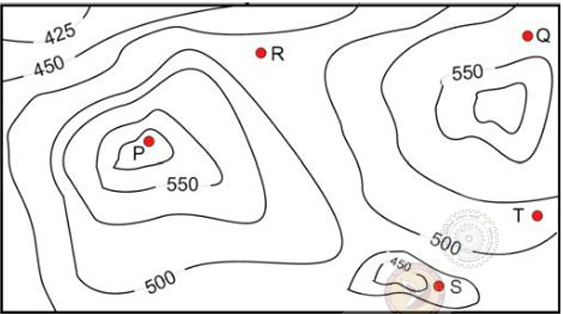
\includegraphics[width=0.4\columnwidth]{figs/q65.png}
        \label{fig:placeholder}
    \end{figure}
    
    \begin{enumerate}
        \begin{multicols}{4}
            \item P, Q
            \item P, Q, T
            \item R, S, T
            \item Q, R, S
        \end{multicols}
    \end{enumerate}
    
    \hfill{\brak{\text{GATE CS 2017}}}
    
\end{enumerate}
\end{document}
